% ALGUNOS PAQUETES REQUERIDOS (EN UBUNTU): %
% ========================================
% %
% texlive-latex-base %
% texlive-latex-recommended %
% texlive-fonts-recommended %
% texlive-latex-extra %
% texlive-science %
% texlive-lang-spanish (en ubuntu 13.10) %
% ******************************************************** %

\documentclass[a4paper]{article}
\usepackage[spanish]{babel}
\usepackage[utf8]{inputenc}
\usepackage{fancyhdr}
\usepackage[pdftex]{graphicx}
\usepackage{sidecap}
\usepackage{caption}
\usepackage{subcaption}
\usepackage{booktabs}
\usepackage{makeidx}
\usepackage{float}
\usepackage{amsmath, amsthm, amssymb}
\usepackage{amsfonts}
\usepackage{sectsty}
\usepackage{wrapfig}
\usepackage{listings}
\usepackage{pgfplots}
\usepackage{enumitem}
\usepackage{hyperref}
\usepackage{listings}
\usepackage{listingsutf8}

\linespread{factor}

\definecolor{mygreen}{rgb}{0,0.6,0}
\definecolor{mygray}{rgb}{0.5,0.5,0.5}
\pgfplotsset{compat=1.3}
\setlist[enumerate]{label*=\arabic*.}
\lstset{
	inputencoding=utf8/latin1,
	language=C++,
	basicstyle=\ttfamily,
	keywordstyle=\bfseries\color{blue},
	stringstyle=\color{red}\ttfamily,
	commentstyle=\color{mygreen}\ttfamily,
	morecomment=[l][\color{magenta}]{\#},
	numbers=left,
	numberstyle=\color{mygray}
}

\usepackage{color} % para snipets de codigo coloreados
\usepackage{fancybox}  % para el sbox de los snipets de codigo

\definecolor{litegrey}{gray}{0.94}

% \newenvironment{sidebar}{%
% 	\begin{Sbox}\begin{minipage}{.85\textwidth}}%
% 	{\end{minipage}\end{Sbox}%
% 		\begin{center}\setlength{\fboxsep}{6pt}%
% 		\shadowbox{\TheSbox}\end{center}}
% \newenvironment{warning}{%
% 	\begin{Sbox}\begin{minipage}{.85\textwidth}\sffamily\lite\small\RaggedRight}%
% 	{\end{minipage}\end{Sbox}%
% 		\begin{center}\setlength{\fboxsep}{6pt}%
% 		\colorbox{litegrey}{\TheSbox}\end{center}}

\newenvironment{codesnippet}{%
	\begin{Sbox}\begin{minipage}{\textwidth}\sffamily\small}%
	{\end{minipage}\end{Sbox}%
		\begin{center}%
		\vspace{-0.4cm}\colorbox{litegrey}{\TheSbox}\end{center}\vspace{0.3cm}}



\usepackage{fancyhdr}
\pagestyle{fancy}
%\renewcommand{\chaptermark}[1]{\markboth{#1}{}}
\renewcommand{\sectionmark}[1]{\markright{\thesection\ - #1}}
\fancyhf{}
\fancyhead[LO]{Sección \rightmark} % \thesection\
\fancyfoot[LO]{\small{Franco Frizzo, Iván Pondal, Manuel Mena, Maximiliano Paz}}
\fancyfoot[RO]{\thepage}
\renewcommand{\headrulewidth}{0.5pt}
\renewcommand{\footrulewidth}{0.5pt}
%\setlength{\hoffset}{-0.8in}
\setlength{\textwidth}{16cm}
\setlength{\hoffset}{-1.1cm}
\setlength{\headsep}{0.5cm}
\setlength{\textheight}{25cm}
\setlength{\voffset}{-0.7in}
\setlength{\headwidth}{\textwidth}
\setlength{\headheight}{13.1pt}
\renewcommand{\baselinestretch}{1.1} % line spacing

\usepackage{caratula}

\newcommand{\ord}{\ensuremath{\operatorname{O}}}
\newcommand{\nat}{\ensuremath{\mathbb{N}}}
\newcommand{\acr}[1]{\textsc{#1}}

% Lemas, definiciones, etc.
\theoremstyle{plain}
  \newtheorem{prop}{Proposición}
  \newtheorem{lema}{Lema}
\theoremstyle{remark}
  \newtheorem{obs}{Observación}
\theoremstyle{definition}
  \newtheorem{defi}{Definición}

% Pseudocódigo
\usepackage[onelanguage, spanish]{algorithm2e}
    % \NoCaptionOfAlgo
    \LinesNumbered\RestyleAlgo{ruled}\IncMargin{1em}\DontPrintSemicolon\SetArgSty{}\SetCommentSty{textsf}\SetFuncSty{textsf}
    \SetKwInput{Input}{Entrada}
    \SetKwInput{Output}{Salida}
    \SetKwProg{For}{para}{ hacer}{fin}
    \SetKwProg{Fn}{función}{:}{fin}

%\lstset{
%    language=C++,
%    basicstyle=\ttfamily,
%    keywordstyle=\color{blue}\ttfamily,
%    stringstyle=\color{red}\ttfamily,
%    commentstyle=\color{ForestGreen}\ttfamily,
%    morecomment=[l][\color{magenta}]{\#}
%}

\begin{document}
\materia{Algoritmos y Estructuras de Datos III}
\submateria{Primer Cuatrimestre de 2016}
\titulo{Episodio II}
%\subtitulo{Grupo: }
\integrante{Franco Frizzo}{013/14}{francofrizzo@gmail.com}
\integrante{Iván Pondal}{078/14}{ivan.pondal@gmail.com}
\integrante{Manuel Mena}{313/14}{manuelmena1993@gmail.com}
\integrante{Maximiliano Paz}{251/14}{m4xileon@gmail.com}

\maketitle
% no footer on the first page
\thispagestyle{empty}

\newpage
\tableofcontents

\newpage
\section{Introducción}
    En el presente trabajo, se detalla la resolución computacional de tres
    problemas algorítmicos, describiendo los modelos utilizados y la
    implementación de las soluciones propuestas. En los tres casos, tras
    demostrar la correctitud de los algoritmos utilizados, se procede a
    deducir una cota teórica para su complejidad temporal, que luego es
    corroborada en forma empírica a través de una serie de experimentos.
    También se verifican hipótesis acerca del comportamiento del algoritmo
    en situaciones de mejor y de peor caso, cuando resulta pertinente.

    Los dos primeros problemas son resueltos por medio de grafos, utilizando
    variantes de conocidos algoritmos para afrontar este tipo de escenarios.
    Para el tercero, por su parte, se utiliza la técnica de programación
    dinámica.

    En los tres casos, se programaron implementaciones de los algoritmos
    en el lenguaje C++, utilizando en varios casos funciones y
    estructuras de datos provistas por la biblioteca estándar del lenguaje.
    Estas implementaciones fueron el objeto de estudio de los experimentos
    mencionados, durante los cuales se tuvieron en cuenta las siguientes
    consideraciones generales:

    \begin{itemize}
    \item Solo se midió el costo temporal de generar las soluciones,
    omitiendo el demandado para la lectura y escritura de los datos.
    \item Para la medición de los tiempos de ejecución, se utilizaron los
    métodos proporcionados por el \emph{header} \texttt{chrono} de la
    biblioteca estándar de C++. Los tiempos fueron medidos en nanosegundos.
    \item Todas las pruebas se corrieron en las computadoras del Laboratorio X
    del Departamento de Computación (\acr{fcen} - \acr{uba}).
    \end{itemize}


\newpage
\section{Ejercicio 1: Una nueva esperanza}

    % Describir detalladamente el problema a resolver dando ejemplos del mismo
    % y sus soluciones.
    \subsection{Descripción del problema}

    \begin{figure}[ht]
        \begin{center}
            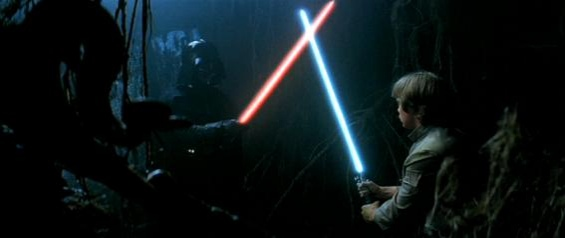
\includegraphics[width=10cm]{imagenes/una_nueva_esperanza.jpg}
            \caption*{``Ese lugar... es fuerte con el lado oscuro de la Fuerza. Un
            dominio del mal es. Dentro tú debes ir.''}
        \end{center}
    \end{figure}

    Como parte de su entrenamiento con el maestro Yoda, Luke Skywalker debe
    recorrer un complejo sistema que consta de $N$ cuevas, conectadas por $M$
    pasadizos. Cada pasadizo une dos cuevas entre sí, formando una red en la
    que siempre existe una forma de llegar desde una cueva hasta cualquier
    otra. Además, no todos los pasadizos son iguales: algunos de ellos son
    especiales, y para atravesarlos Luke deberá enfrentarse a sus mayores
    miedos. Recorrer cualquier pasadizo le demanda a Luke exactamente un
    minuto.

    Partiendo de una cueva etiquetada con el número $0$, Luke debe llegar en
    el menor tiempo posible a la cueva número $N-1$, donde lo espera Yoda.
    Sin embargo, su entrenamiento no estará completo hasta no haber pasado al
    menos por dos pasadizos especiales. Está permitido recorrer el mismo
    pasadizo más de una vez.

    Se pide implementar un algoritmo que determine el menor tiempo posible que
    le demandará a Luke completar su entrenamiento, y la secuencia de cuevas
    que deberá recorrer para lograrlo, con una complejidad temporal de
    $\ord(N + M)$.

    \vspace{1.25em}

    \textbf{Formato de entrada}: La primera línea consta de un entero positivo
    \texttt{N}, que indica la cantidad de cuevas, y un entero positivo
    \texttt{M}, que indica la cantidad de pasadizos. A continuación de esta
    línea siguen \texttt{M} líneas con enteros \texttt{Ai}, \texttt{Bi} y
    \texttt{Ei}, cada una de ellas correspondiente a un pasadizo, donde
    \texttt{Ai} y \texttt{Bi} son enteros (entre $0$ y $N-1$ inclusive) que
    indican los extremos del mismo, mientras que \texttt{Ei} indica
    el tipo de pasadizo ($0$ para los pasadizos comunes y $1$ para los
    especiales). Es decir, el formato de la entrada es el siguiente:

    \begin{verbatim}
    N M
    A0 B0 E0
    A1 B1 E1
    ...
    AM-1 BM-1 EM-1\end{verbatim}

    \vspace{.8em}

    \textbf{Formato de salida}: Debe devolverse una primera línea conteniendo
    la cantidad de minutos (\texttt{T}) que durará el entrenamiento de Luke,
    y una segunda línea con la lista ordenada de las cuevas (\texttt{I1},
    \texttt{I2}, \dots, \texttt{I(T-1)}) que deberá recorrer para
    completarlo, omitiendo la salida desde la cueva $0$ y la llegada a la
    cueva $N-1$. El formato requerido es el siguiente:

    \begin{verbatim}
    T
    I1 I2 ... I(T-1)\end{verbatim}

    \vspace{.8em}

    A continuación se incluyen, a modo de ejemplo, una posible entrada y una
    salida correcta para la misma:

    \vspace{.5em}
    \begin{tabular}{l @{\hskip 4em} l}
    \textbf{Entrada} & \textbf{Salida} \\
    \texttt{5 6}     & \texttt{3}      \\
    \texttt{0 1 0}   & \texttt{2 3}    \\
    \texttt{0 2 1}   &                 \\
    \texttt{0 4 0}   &                 \\
    \texttt{1 3 0}   &                 \\
    \texttt{2 3 0}   &                 \\
    \texttt{3 4 1}   &                 \\
    \end{tabular}
    \vspace{.5em}

    Es importante observar que puede haber más de una salida distinta válida.

    % Explicar de forma clara, sencilla, estructurada y concisa, las ideas
    % desarrolladas para la resolución del problema. Utilizar pseudocódigo y
    % lenguaje coloquial (no código fuente). Justificar por qué el
    % procedimiento resuelve efectivamente el problema.
    \subsection{Solución propuesta}

	\subsubsection{Modelo}

	Para resolver este problema se exigía encontrar el camino que recorriera al
	menos 2 pasillos especiales con un costo mínimo de tiempo, donde el mismo se
	define como el total de pasillos atravesados. Lo primero que se realizó fue
	modelar el problema con grafos dado que el mismo tenía características que
	sugerían que para la resolución iba a ser necesario calcular un camino mínimo de algún tipo.

	La primer idea de representación con grafos fue tener las cuevas como nodos y
	los pasillos como aristas. Sin embargo, quedaban aquí sin contemplar los
	pasillos especiales. Para subsanar esto, cada arista contiene además una bandera
	indicando si es o no un pasillo especial.

	Este grafo era una forma de modelar el problema donde aún no quedaba claro
	cómo resolver el ejercicio. Si se buscaba el camino mínimo del punto inicial
	al resto de las cuevas no existía ninguna garantía de que se cumpliera la
	condición de haber recorrido al menos 2 pasillos especiales.

	Para la versión final del modelo, lo que se hizo fue generar copias del
	grafo descrito anteriormente, teniendo como diferencia entre estos su
	\emph{estado}. El estado lo que indicará es para cada una de estas copias la
	cantidad de caminos especiales recorridos.

	Se tienen tres grafos, uno para cada uno de los siguientes estados:

	\begin{enumerate}
		\item{No se recorrió ningún pasillo especial.}
		\item{Se recorrió un pasillo especial.}
		\item{Se recorrieron al menos dos pasillos especiales.}
	\end{enumerate}

	\begin{figure}[H]
		\centering
		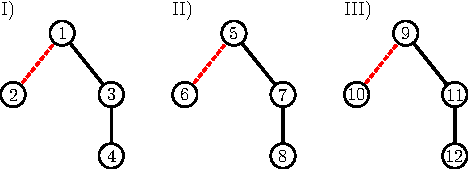
\includegraphics{imagenes/ej1_modelo_1.pdf}
		\caption{Visualización de los grafos con las aristas rojas representando un pasillo especial.}
		\label{ej1:fig_1}
	\end{figure}

	Una posible observación es que por más que cada grafo representa el mismo
	conjunto de cuevas y pasillos, para cada estado se utilizan
	números distintos para identificar cada nodo. Esto se debe a que ésta será
	la forma de identificar en qué estado se encuentra cada nodo. Se define la
	siguiente función donde $V$ es el número de nodo y $N$ el total de cuevas
	dado por la entrada:

	\begin{equation*}
		estado(V) =
		\begin{cases}
			1 & , V \leq N \\
			2 & , N < V \leq 2 * N \\
			3 & , 2 * N < V \leq 3 * N
		\end{cases}
	\end{equation*}

	Teniendo esta representación, se procede a explicar el algoritmo y
	solución desarrollada. Existen dos objetivos: que Luke atraviese al menos 2
	caminos especiales, que el camino que tome para lograr eso sea mínimo. Para
	lo segundo, como las aristas no poséen pesos, se puede utilizar
	\emph{Breadth First Search}, que permite obtener la distancia de un nodo
	cualquiera hacia el resto. Sin embargo esto solo no alcanza, ya que es
	requisito el recorrer al menos 2 caminos especiales. Para cumplir con esta
	condición se introduce una ligera modificación al \emph{BFS}: si un vecino
	se accede cruzando un pasillo especial, el nodo correspondiente en el estado
	siguiente se marca como visitado y se encolan sus vecinos.

	De esta manera lo que se logra es que en cuanto se realiza un cambio de
	estado (el salto a un vecino mediante un pasillo especial), se permite que
	el \emph{BFS} recorra cuevas que ya había visitado, con la diferencia de que
	cuenta con el hecho de que atravesó al menos un pasillo especial.

	Siguiendo esta lógica se obtiene la distancia de una cueva al resto en
	alguno de sus posibles estados. En particular, tomando el grafo
	correspondiente al estado donde se recorrieron al menos 2 pasillos
	especiales, la distancia hasta el nodo que equivale al $N - 1$ es la del camino mínimo
	pedido por el enunciado.

	A continuación se presenta el efecto de cada iteración del algoritmo sobre el grafo
	presentado en la Figura \ref{ej1:fig_1}:

	\begin{figure}[H]
		\centering
		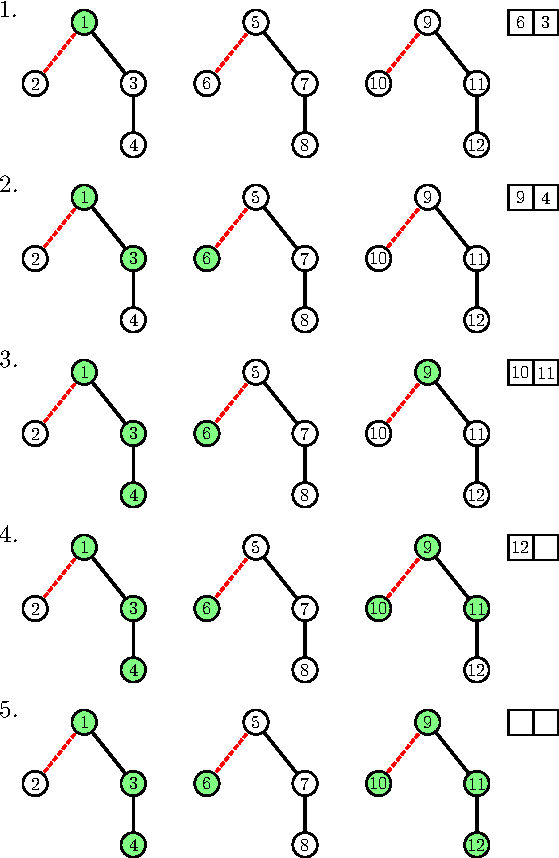
\includegraphics{imagenes/ej1_modelo_2.pdf}
		\caption{Visualización del \emph{BFS} marcando con verde los nodos
		visitados.}
		\label{ej1:bfs}
	\end{figure}

	Esta ejecución genera el siguiente árbol de caminos mínimos, donde se puede
	observar que se obtiene la distancia al nodo 12 que es el equivalente al $N
	- 1$ en el grafo donde se recorrieron al menos 2 pasillos especiales:

	\begin{figure}[H]
		\centering
		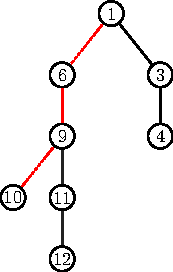
\includegraphics{imagenes/ej1_modelo_3.pdf}
		\caption{Árbol de caminos mínimos del nodo inicial al resto.}
	\end{figure}

	Una vez que se tiene este árbol de caminos mínimos, para armar la solución se trepa
	desde el nodo $N - 1$ (con $estado(N - 1) = 3$) hasta la
	raiz, traduciendo el índice de cada nodo al de su equivalente en el grafo
	original. Por ejemplo, el nodo 12 es en realidad la cueva 4 con $estado(12) =
	3$, por lo tanto a la hora de armar el camino se lo traducirá a 4.

	Habiendo introducido la idea detrás de la solución desarrolada, se procede a
	demostrar que esto efectivamente funciona, es decir que con esta
	modificación al \emph{BFS} siempre se encontrará un camino mínimo hasta la
	cueva $N - 1$ habiendo recorrido al menos 2 pasillos especiales.

	\subsubsection{Demostración de correctitud}

	Para probar que se cumple lo pedido, primero se realizará inducción sobre los ciclos
	del \emph{BFS} modificado buscando demostrar que al finalizar, se obtienen
	los caminos mínimos teniendo en cuenta la condición de pasadizos especiales
	recorridos.

	\subsubsection*{Correctitud del ciclo}

	El invariante a demostrar será el siguiente: al terminar el ciclo $k$ del
	\emph{BFS} modificado se obtienen todos los nodos a distancia a lo sumo
	$k$ del inicial en alguno de los estados posibles. Esto se probará
	mediante inducción en los ciclos del algoritmo.

	~

	\textbf{Caso base: } $k = 1$

	En el caso base se tiene únicamente el nodo inicial marcado como
	visitado con distancia 0. Como se trata del nodo inicial, se encuentra en el primer estado ya que
	no se recorrieron pasadizos especiales. Por lo tanto, existen dos posibles
	formas de accionar con respecto a sus vecinos:

	\begin{enumerate}
		\item{
			El vecino está conectado mediante un pasadizo común, con lo cual en
			el grafo del nodo inicial se lo marca con distancia 1 y encolan sus
			vecinos.
		}
		\item{
			El vecino está conectado mediante un pasadizo especial, por lo tanto
			en el grafo en el estado siguiente, es decir en el que se cuenta con
			que se recorrió un pasadizo especial, se lo marca con distancia 1 y
			encolan sus vecinos.
		}
	\end{enumerate}

	De esta forma una vez finalizada la iteración $k = 1$ se obtienen todos los
	nodos que están a distancia 1 del nodo inicial.

	~

	\textbf{Paso inductivo: } $k > 1$

	Como hipótesis inductiva se cuenta con que vale el invariante para $k - 1$,
	por lo tanto se tiene la distancia para todos los nodos a lo sumo
	a distancia $k - 1$ para alguno de los estados descritos y además se
	tienen encolados para visitar los que están a distancia $k$.

	Ahora acá existen distintas posibilidades por el hecho de que a diferencia
	del caso base, los nodos encolados no tienen por qué necesariamente
	encontrarse en el primer estado. Pueden haber nodos pertenecientes al
	segundo como tercer estado (un pasadizo especial o al menos dos recorridos).

	Es entonces necesario probar que en cada caso el invariante seguirá
	valiendo:

	\begin{enumerate}
		\item{
			El nodo encolado pertenece al primer estado. En este escenario, al
			igual que con el caso base existen dos posibles formas de operar en
			función de si se accede a un vecino mediante una arista especial:

			\begin{enumerate}
				\item{
					El vecino está conectado mediante un pasadizo común, con lo
					cual en el grafo del primer estado se observa si ya se
					encuentra marcado. En caso de no estar marcado, en ese
					mismo grafo se le asigna la distancia $k$ y encolan sus
					vecinos.
				}
				\item{
					El vecino está conectado mediante un pasadizo especial, con
					lo cual en el grafo del segundo estado se observa si ya se
					encuentra marcado. En caso de no estar marcado en ese mismo
					grafo se le asigna la distancia $k$ y encolan sus vecinos.
				}
			\end{enumerate}
		}
		\item{
			El nodo encolado pertence al segundo estado. Nuevamente existen dos
			posibles formas de operar en función de si la arista que lo conecta
			a un vecino es especial:

			\begin{enumerate}
				\item{
					El vecino está conectado mediante un pasadizo común, con lo
					cual en el grafo del segundo estado se observa si ya se
					encuentra marcado. En caso de no estar marcado, en ese mismo
					grafo se le asigna distancia $k$ y encolan sus vecinos.
				}
				\item{
					El vecino está conectado mediante un pasadizo especial, con
					lo cual en el grafo del tercer estado se observa si ya se
					encuentra marcado. En caso de no estar marcado en ese mismo
					grafo se le asigna la distancia $k$ y encolan sus vecinos.
				}
			\end{enumerate}
		}
		\item{
			Por último, en caso de que el nodo encolado pertenezca al tercer
			estado existe una única manera de proceder, ya que en caso de que un
			vecino se encuentre conectado mediante una arista especial ya no hay
			un estado sucesor.

			Si en el grafo del tercer estado alguno de los vecinos no se
			encuentra marcado, se le asigna distancia $k$ y es encolado para ser
			visitado.
		}
	\end{enumerate}

	Habiendo contemplado cada escenario posible es posible afirmar que al
	finalizar la iteración $k$ con $k > 2$ se obtienen todos los nodos a
	distancia $k$ para alguno de los estados posibles.

	Por inducción en los ciclos del algoritmo, se demuestra que para
	toda iteración se cumple el invariante, con lo cual al finalizar se obtiene
	la distancia de todos los nodos para alguno de los estados descritos.

	Queda probar entonces que si existe al menos una arista especial entonces
	siempre se obtendrá la distancia hasta el nodo $N - 1$ en el tercer estado,
	es decir el mínimo camino tal que se atraviesan al menos dos caminos
	especiales.

	Para probar que esto vale, se demostrará que el grafo vinculado al tercer
	estado, tendrá todos sus nodos marcados con su respectiva distancia.

	\subsubsection*{Existencia de un camino mínimo al nodo $N - 1$ en el tercer
	estado}

	Como se dijo previamente, se probará que todo nodo pertenciente al tercer
	estado se encuentra marcado con su respectiva distancia. Supongamos que esto
	no es cierto, que existe al menos un nodo sin marcar. Esto podría ser
	resultado de uno de los siguientes escenarios:

	\begin{itemize}
		\item{Nunca se salta al tercer estado, en este caso resultando en que no
			haya ningún nodo marcado en el mismo.}
		\item{Se llega al tercer estado pero no se recorren todos sus nodos.}
	\end{itemize}

	Si se considera el primer escenario, esto implica que jamás se saltó del
	segundo al tercer estado. Sin embargo para que esto ocurriese se debería
	cumplir una de las siguientes condiciones: jamás se saltó al segundo estado
	o ningún nodo del segundo estado tiene un vecino conectado mediante una
	arista especial. Es fácil ver que ninguna de estas condiciones se cumplen.

	La primera, como se asume que siempre existe al menos un pasadizo especial,
	por el comportamiento del \emph{BFS} modificado eventualmente se
	encontrará un nodo cuyo vecino está conectado por una arista especial y en el
	grafo del segundo estado este vecino no estará marcado, con lo cual lo
	marcará y encolará sus vecinos saltando de esta forma al segundo estado.

	Lo segundo, que ningún nodo del segundo estado tenga un vecino conectado
	mediante un pasadizo especial, carece de sentido por el hecho de que el
	grafo vinculado con el segundo estado es una copia del primero. Entonces, si
	del primero se salta al segundo, en este estado el nodo seguro tendrá como
	vecino el nodo del que saltó, también conectado mediante una arista
	especial.

	Por lo tanto habiendo visto que ninguna de estas condiciones se cumplen
	queda demostrado que el primer escenario nunca puede suceder, ya que si se
	llega al segundo estado y además se cuenta con que habrán vecinos conectados
	mediante aristas especiales esto significa que van a existir saltos al
	tercer estado.

	Queda entonces el segundo escenario, se llega al tercer estado pero no se
	recorren todos sus nodos. Esto es algo que podría suceder en el primer o
	segundo estado (véase Figura \ref{ej1:bfs}) pero no en el tercero.

	Si quedan nodos sin marcar en el tercer grafo es porque los mismos jamás
	fueron encolados para visitarlos. Ya se demostró que al tercer estado se
	salta en algún momento, con lo cual al menos uno de los nodos de
	seguro va a estar marcado. Luego por la descripción del \emph{BFS}
	modificado tenemos que un nodo en el tercer estado ya no salta a otro grafo,
	con lo cual todos los vecinos no marcados son visitados. De esta forma no
	hay manera que queden nodos sin visitar, ya que o bien están marcados de
	forma directa como vecinos de un nodo del segundo estado, o son alcanzados por
	el avance del \emph{BFS} de alguno de los nodos provenientes de un salto del segundo estado.

	Así se prueba entonces que ninguno de los escenarios planteados pueden
	suceder, con lo cual todos los nodos en el tercer estado están marcados y
	poséen un camino mínimo hasta el nodo inicial en el primer estado. Como
	consecuencia de esto, en particual de seguro existe un camino mínimo del
	nodo incial en el primer estado al nodo $N - 1$ en el tercer estado.

    % Deducir una cota de complejidad temporal del algoritmo propuesto (en
    % función de los parámetros que se consideren correctos) y justificar por
    % qué el algoritmo la cumple. Utilizar el modelo uniforme.
    \subsection{Complejidad teórica}
    Crear el vector de representación para los estados de los nodos e instaciarlo en $-1$ tiene un costo de $O(3N)$.  

    Se encola el primer nodo, luego por cada nodo desencolado, se recorre sus vecinos, si es camino especial se ira al nodo del siguiente nivel, si ya fue visitado no se agrega a la cola ($O(1)$).En el peor de los casos por cada nodo de cada nivel, se recorre todas sus aristas y por cada arista se hace algo de complejidad $O(1)$, Entonces nos queda $O(3M)$.

    Por último se arma el camino óptimo partiendo del nodo destino en el tercer nivel y se va agregando de donde venia y me muevo a él hasta llegar al nodo incial, esto tiene complejidad $O(N + N')$, donde $N' < N$, porque si el camino minimo del nodo inicial al nodo final tiene uno ó más caminos especiales nos queda $O(N)$, caso contrario tendria ir a un camino especial ($O(N')$) y luego a el nodo destino ($O(N)$) .

    La complejidad total nos queda $O(3N + 3M + N + N') = O(M)$, ya que como el grafo es conexo como minimo tengo $N-1$ aristas osea $M > N-1$.

    % Realizar experimentación para medir la performance, usando un conjunto
    % de casos de test que permitan observar los tiempos de ejecución en
    % función de los parámetros de entrada, tanto para instancias aleatorias
    % (detallando cómo fueron generadas) como para instancias particulares
    % (peor/mejor caso, por ejemplo). Presentar en forma gráfica una
    % comparación entre los tiempos medidos y la complejidad teórica y extraer
    % conclusiones.
    \subsection{Experimentación}

    % Ejemplo de gráfico para reutilizar:
    % \begin{figure}[H]
    %     \centering
    %     \caption{}
    %     \label{fig:exp1:tiempo_base}
    %     \begin{tikzpicture}
    %         \begin{axis}[
    %                 title={},
    %                 xlabel={Tamaño de entrada ($N$)},
    %                 ylabel={Tiempo de ejecución (nanosegundos)},
    %                 scaled x ticks=false,
    %                 scaled y ticks=false,
    %                 enlargelimits=0.05,
    %                 width=0.5\textwidth,
    %                 height=0.5\textwidth,
    %                 legend pos=south east,
    %                 legend cell align=left,
    %                 xmin=1
    %             ]
    %             \addplot[color=black]
    %                 table[x index=0,y index=1]
    %                 {../exp/kaioKenOutput};
    %             \addplot[color=red]
    %                 table[x index=0, y expr={x*ln(x)*\constante}]
    %                 {../exp/kaioKenOutput};
    %             \legend{$T$, $c*N*log(N)$}
    %         \end{axis}
    %     \end{tikzpicture}
    % \end{figure}


\newpage
\section{Ejercicio 2: El Imperio contraataca}

    % Describir detalladamente el problema a resolver dando ejemplos del mismo y sus soluciones.
    \subsection{Descripción del problema}

    \begin{figure}[ht]
        \begin{center}
            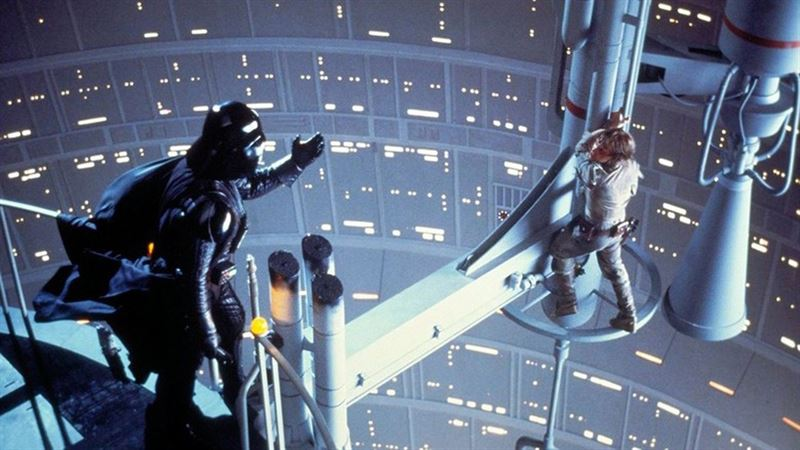
\includegraphics[width=10cm]{imagenes/el_imperio_contraataca.jpg}
            \caption{¡Prestame atención a mí, soy tu padre!}
        \end{center}
    \end{figure}

    Luke debe informarle a todos sus aliados para que estén al tanto del contraataque del Imperio. Parte del planeta Hoth, conocido como planeta 0, y quiere que la noticia llegue a todos los planetas.

    En cada planeta hay infinitos halcones milenarios. Los halcones milenarios consumen una determinada de combustible cada un millón de kilómetros.

    Una vez que un halcón milenario llega a un planeta, de éste pueden salir cualquier cantidad de halcones para seguir advirtiendo a los rebeldes de otros planetas.

    Los halcones milenarios no pueden viajar por cualquier lado, solo por determinadas rutas espaciales. Cada ruta conecta exactamente dos planetas, y recorrer cada ruta consume una determinada cantidad de combustible. Además, se sabe que existe al menos una forma de llegar desde cualquier planeta a cualquier otro a través de rutas espaciales.

    Se pide encontrar cuál es la mínima cantidad de combustible necesaria para entregar el mensaje en todos los planetas. Además, se debe indicar de qué planeta proviene la nave que entrega el mensaje, para cada planeta excepto el 0.

    Se pide que el algoritmo tenga una complejidad temporal $\ord(M$ log $M)$. \\

    \textbf{Formato de entrada}: La primera línea consta de un entero positivo \texttt{N}, que indica la cantidad de planetas, y un entero positivo M, que indica la cantidad de rutas espaciales. A continuación de esta línea siguen \texttt{M} líneas con enteros \texttt{Ai}, \texttt{Bi} y \texttt{Li}, siendo \texttt{Ai} y \texttt{Bi} los extremos de la ruta y \texttt{Li} la cantidad de litros que se gastan al recorrer esa ruta ($0 \leq \mathtt{Ai} \neq \mathtt{Bi} \leq N-1$). La entrada contará con el siguiente formato:

    \begin{verbatim}
    N M
    A0 B0 L0 
    A1 B1 L1 
    ...
    AM-1 BM-1 LM-1
    \end{verbatim}

    \textbf{Formato de salida}: La primera línea debe contener la cantidad mínima de litros \texttt{L} necesarios para informar a toda la alianza sobre esta noticia, seguida de $N-1$ líneas que indican desde qué planeta se viaja para informar de la situación a cada planeta (el vecino inmediato desde el cual se viaja). El formato debe ser el siguiente:
    
    \begin{verbatim}
    L
    I1
    I2
    ...
    IN-1
    \end{verbatim}

    indicando que al planeta \texttt{i} se le informa de la situación con una nave que parte del planeta \texttt{Ii}.

    A continuación se incluyen, a modo de ejemplo, una posible entrada y una
    salida correcta para la misma:

    \begin{tabular}{ll}
    \textbf{Entrada} & \textbf{Salida} \\
    \texttt{4 4}     & \texttt{4}      \\
    \texttt{0 1 1}   & \texttt{0}      \\
    \texttt{1 2 2}   & \texttt{1}      \\
    \texttt{1 3 5}   & \texttt{2}      \\
    \texttt{2 3 1}   &                 \\
    \end{tabular}

    Es importante observar que pueden haber más de una salida distinta válida.

    % Explicar de forma clara, sencilla, estructurada y concisa, las ideas
    % desarrolladas para la resolución del problema. Utilizar pseudocódigo y
    % lenguaje coloquial (no código fuente). Justificar por qué el
    % procedimiento resuelve efectivamente el problema.
    \subsection{Solución propuesta}

    El hecho de que los planetas se encontraran unidos mediante rutas, y que
    cada una de ellas conectara exactamente dos planetas, permitió encarar la
    resolución del problema modelando el sistema planetario mediante un
    grafo, donde cada planeta es un vértice y cada ruta es un eje.

    Para representar los distintos costos de utilizar una u otra ruta
    espacial, se consideró un grafo ponderado, utilizando como peso de cada
    eje la cantidad de combustible que cuesta recorrer la ruta
    correspondiente. Por otra parte, el hecho de que siempre exista forma de
    viajar entre dos planetas equivale a decir que el grafo es conexo.

    Sea $G$ el grafo cuyo conjunto de vértices son los planetas y su conjunto
    de aristas, las rutas espaciales. Bajo este modelo, el problema que busca
    resolverse es hallar un subgrafo $T$ de $G$, de forma tal que:
    \begin{itemize}
        \item Todos los nodos de $G$ sean nodos de $T$.
        \item Llamando $v_0 \in V(G)$ al planeta Hoth, exista en $T$ un camino
        entre $v_0$ y cualquier otro planeta. Dado que $T$ es un grafo no
        dirigido, esto equivale a pedir que $T$ sea conexo.
        \item La suma de los pesos de todos los ejes $T$ sea mínima con
        respecto a todos los subgrafos de $G$ que cumplen los dos puntos
        anteriores.
    \end{itemize}


    \begin{lema}
    Todo subgrafo $T \subseteq G$ que cumpla con los tres puntos anteriores
    es un árbol generador mínimo de $G$.
    \end{lema}
    \begin{proof}

    \end{proof}

    % Deducir una cota de complejidad temporal del algoritmo propuesto (en
    % función de los parámetros que se consideren correctos) y justificar por
    % qué el algoritmo la cumple. Utilizar el modelo uniforme.
    \subsection{Complejidad teórica}

    % Realizar experimentación para medir la performance, usando un conjunto
    % de casos de test que permitan observar los tiempos de ejecución en
    % función de los parámetros de entrada, tanto para instancias aleatorias
    % (detallando cómo fueron generadas) como para instancias particulares
    % (peor/mejor caso, por ejemplo). Presentar en forma gráfica una
    % comparación entre los tiempos medidos y la complejidad teórica y extraer
    % conclusiones.
    \subsection{Experimentación}

    % Ejemplo de gráfico para reutilizar:
    % \begin{figure}[H]
    %     \centering
    %     \caption{}
    %     \label{fig:exp1:tiempo_base}
    %     \begin{tikzpicture}
    %         \begin{axis}[
    %                 title={},
    %                 xlabel={Tamaño de entrada ($N$)},
    %                 ylabel={Tiempo de ejecución (nanosegundos)},
    %                 scaled x ticks=false,
    %                 scaled y ticks=false,
    %                 enlargelimits=0.05,
    %                 width=0.5\textwidth,
    %                 height=0.5\textwidth,
    %                 legend pos=south east,
    %                 legend cell align=left,
    %                 xmin=1
    %             ]
    %             \addplot[color=black] table[x index=0,y index=1]{../exp/kaioKenOutput};
    %             \addplot[color=red] table[x index=0, y expr={x*ln(x)*\constante}]{../exp/kaioKenOutput};
    %             \legend{$T$, $c*N*log(N)$}
    %         \end{axis}
    %     \end{tikzpicture}
    % \end{figure}


\newpage
\section{Ejercicio 3: El retorno del jedi}

    % Describir detalladamente el problema a resolver dando ejemplos del mismo y sus soluciones.
    \subsection{Descripción del problema}

    \begin{figure}[ht]
        \begin{center}
            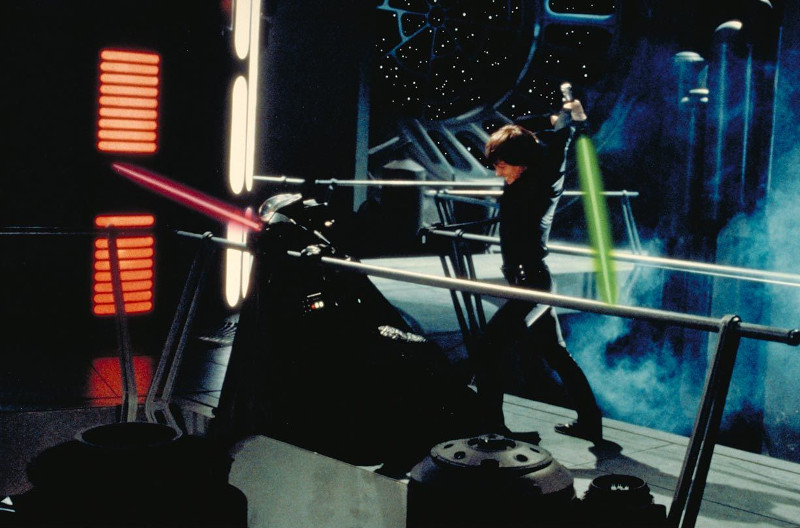
\includegraphics[width=10cm]{imagenes/el_retorno_del_jedi.jpg}
			\caption*{``Muchos son los caminos que conllevan al lado oscuro, el
			odio lleva a la ira, la ira lleva a la venganza''.}
        \end{center}
    \end{figure}

	Luke debe enfrentar a su padre. Para ello debe moverse por una grilla,
	arrancando en la esquina superior izquierda para terminar en la opuesta,
	donde aguarda Darth Vader. Cada casilla de la grilla tiene una altura
	asociada, donde dependiendo de la diferencia en altura entre el casillero
	actual de Luke y su destino le costará más o menos energía moverse. Además
	se tiene la condición de que Luke únicamente puede avanzar hacia abajo o
	hacia la derecha, dado que considera un acto de cobardía retroceder sobre
	sus pasos. El objetivo es encontrar y devolver el camino donde Luke gasta la
	menor cantidad de energía en alcanzar su destino.

	Formalizando el problema, se tiene una grilla $G$ rectangular de dimensiones $N \times
	M$ donde Luke comienza en la posición $(1, 1)$ y desea llegar a $(N, M)$.
	Sea $G_{ij}$ con $1 \leq i \leq N$ y $1 \leq j \leq M$ la altura de cada
	casillero, $H$ el nivel de entrenamiento de Luke y $\Delta$ la
	diferencia de altura entre el casillero actual y el próximo, el costo de
	energía para cada movimiento se calcula de la siguiente manera: nulo si $|\Delta|
	\leq H$, $|\Delta| - H$ en caso contrario. La condición de que Luke no pueda
	retroceder es equivalente a decir que únicamente puede moverse de forma
	creciente en $i$ o $j$.

	El formato de entrada para el problema es el siguiente, donde la primer
	línea posee las dimensiones de la grilla y el nivel de entrenamiento de
	Luke, y las siguientes $N$ entradas contienen $M$ elementos donde cada uno
	representa la altura del casillero correspondiente.

	~
	\begin{center}
		\begin{tabular}{cccc}
			$N$ & $M$ & $H$ & \\
			$G_{11}$ & $G_{12}$ & $\dots$ & $G_{1M}$ \\
			$G_{21}$ & $G_{22}$ & $\dots$ & $G_{2M}$ \\
			$\vdots$ & & & \\
			$G_{N1}$ & $G_{N2}$ & $\dots$ & $G_{NM}$ \\
		\end{tabular}
	\end{center}

	~

	La salida está compuesta por una primer línea con el costo del camino
	seleccionado y $N + M - 2$ líneas con la dirección ($X$ o $Y$) a tomar en cada paso para
	realizar el mismo. Cabe aclarar que $X$ implica avanzar una filas e $Y$
	una columna.

	A continuación se presenta un ejemplo de entrada con su salida
	correspondiente:

	~

	\begin{figure}[H]
		\centering
		\begin{minipage}[t]{0.25\textwidth}
			\begin{tabular}[t]{ccc}
				\multicolumn{3}{l}{\textbf{Entrada}} \\
				\texttt{3} & \texttt{3} & \texttt{1} \\
				\texttt{4} & \texttt{-2} & \texttt{-1} \\
				\texttt{6} & \texttt{7} & \texttt{-5} \\
				\texttt{0} & \texttt{3} & \texttt{4} \\
			\end{tabular}
		\end{minipage}
		\begin{minipage}[t]{0.10\textwidth}
			\begin{tabular}[t]{l}
				\textbf{Salida} \\
				\texttt{4} \\
				\texttt{X} \\
				\texttt{Y} \\
				\texttt{X} \\
				\texttt{Y} \\
			\end{tabular}
		\end{minipage}
	\end{figure}

	\begin{figure}[H]
		\centering
		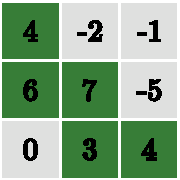
\includegraphics{imagenes/ej3_grilla_1.pdf}
		\caption{Camino de menor costo.}
	\end{figure}

    % Explicar de forma clara, sencilla, estructurada y concisa, las ideas desarrolladas para la resolución del problema. Utilizar pseudocódigo y lenguaje coloquial (no código fuente). Justificar por qué el procedimiento resuelve efectivamente el problema.
    \subsection{Solución propuesta}

	Para la resolución de este ejercicio se utilizó programación dinámica dado
	que el mismo presenta solapamiento de subproblemas y es posible definir una
	formulación recursiva que lo resuelva haciendo uso del principio de
	optimalidad.

	Dada una entrada con entrenamiento $H$, la siguiente función modela la solución al
	problema:

	\begin{equation*}
		f(N, M) = \text{Costo mínimo de $(1, 1)$ a $(N, M)$ para Luke con entrenamiento $H$}
	\end{equation*}

	Luego se plantea la recurrencia donde es posible visualizar qué valores
	podrían guardarse para no tener que recalcularlos (solapamiento).
	Antes por comodidad se define la siguiente función $g$ para calcular el costo de cada salto:

	\begin{equation*}
		g(i, j, i', j') =
		\begin{cases}
			|G_{ij} - G_{i'j'}| - H & \text{si } |G_{ij} - G_{i'j'}| > H \\
			0 & \text{caso contrario}
		\end{cases}
	\end{equation*}

	Ahora sí se define la versión recursiva del ejercicio de la siguiente manera:

	\begin{align*}
		f(1, 1) &= 0 \\
		f(1, j) &= g(1, j, 1, j - 1) + f(1, j - 1) \\
		f(i, 1) &= g(i, 1, i - 1, 1) + f(i - 1, 1) \\
		f(i, j) &= \text{mín}\left \{ f(i - 1, j) + g(i, j, i - 1, j), f(i, j - 1) + g(i, j, i, j - 1) \right \} \\
	\end{align*}

	La función propuesta devuelve el valor que minimiza la suma
	entre la llamada recursiva en los posibles casilleros anteriores más el
	costo de su respectivo salto. Esto requiere que se contemplen por separado
	los bordes por el hecho de que tienen un único casillero anterior posible.
	El caso base es $f(1, 1) = 0$ dado que es el punto de partida del
	problema, su costo asociado es nulo. Lo importante aquí es que cuando se tienen
	dos posibles antecesores es necesario contemplar tanto el valor de la
	función como el costo del salto.

	Esta recurrencia es una solución al problema únicamente si se cumple el principio
	de optimalidad. Si el mismo se cumple, entonces las subsoluciones al problema son
	óptimas, pudiendo así operar y reutilizar valores que se tiene la certeza
	que son el mejor camino a tomar. Los subproblemas para este ejercicio están
	representados por el costo mínimo hasta cualquier $(i, j)$ dado por $f(i,
	j)$. Por lo tanto a continuación se procederá a demostrar que vale tal
	propiedad.

	\subsubsection*{Optimalidad de subproblemas}

	La idea detrás de la recurrencia es que la solución de encontrar el camino
	de menor costo hasta $(N, M)$ se puede pensar como la decisión entre tomar
	el mejor camino a $(N - 1, M)$ o $(N, M - 1)$ más el salto final. Para poder
	usar esto es necesario entonces demostrar que el camino seleccionado hasta
	$(N - 1, M)$ o $(N, M - 1)$ sea óptimo.

	Este es el concepto de subproblemas, el hecho de considerar todo camino a
	$(i, j)$ como una subsolución al problema principal. Para probar que con la
	función recursiva se obtienen estas subsoluciones óptimas se realiza
	inducción sobre $N$ y $M$.

	~

	\textbf{Caso base: } $N = M = 1$

	Por definición de la recurrencia, $f(1, 1) = 0$ lo cual es válido ya que si
	Luke no tiene que moverse en ninguna dirección, no necesita realizar ningún
	salto manteniendo intacto su nivel de energía. Queda así demostrada la
	validez del caso base.

	~

	\textbf{Paso inductivo}

	Para el paso inductivo es necesario contemplar por separado los casos
	bordes, con lo cual se analizarán tres situaciones posibles.

	\begin{enumerate}
		\item{
			\textbf{Columna lateral izquierda: } $f(i, 1)$ con $1 < i < N$

			Como hipótesis inductiva, se asume $f(i - 1, 1)$ óptimo.

			Luke únicamente puede avanzar en orden creciente tanto en $i$
			o en $j$, la única forma de acceder a los casilleros de la primer
			columna es avanzando sólo en $i$, ya que en con moverse
			una posición en $j$ ya le resulta imposible retroceder y llegar a
			estos.

			Estos caminos están definidos por $f(i, 1) = g(i, 1, i - 1, 1) + f(i
			- 1, 1)$ donde se toma el costo del camino hasta una posición atrás
			en $i$ y se le suma el valor del salto. Como sólo es posible llegar
			a través del casillero anterior ($i - 1$, 1), y por hipótesis inductiva
			dijimos que $f(i - 1, 1)$ era óptimo, al sumarle el valor del salto
			se obtiene la subsolución $f(i, 1)$.
		}
		\item{
			\textbf{Fila superior: } $f(1, j)$ con $1 < j < M$

			Como hipótesis inductiva, se asume $f(1, j - 1)$ óptimo.

			Similar al punto anterior, por la restricción que tiene Luke para
			desplazarse, estas posiciones sólo pueden accederse avanzando sólo
			en $j$ desde el casillero inicial.

			Los costos están definidos por $f(1, j) = g(1, j, 1, j - 1) + f(1, j
			- 1)$, que toma el costo del camino hasta una posición atrás en $j$
			y le suma el valor del salto. Dado que sólo es posible llegar desde
			$(1, j - 1)$ y por hipótesis inductiva $f(1, j - 1)$ es óptimo, al
			sumarle el salto se obtiene la subsolución $f(1, j)$.
		}
		\item{
			\textbf{Elementos restantes: } $f(i, j)$ con $1 < i \leq N$ y $1 < j \leq M$

			Como hipótesis inductiva, se asumen $f(i - 1, j)$ y $f(i, j - 1)$
			óptimos.

			Habiendo considerado ya los casos bordes, ahora es posible para el
			resto de casilleros $(i, j)$ dar su camino de menor costo, ya que
			para llegar a uno de ellos hay sólo dos opciones: se salta de $(i -
			1, j)$ o de $(i, j - 1)$. Luke no puede moverse en diagonal ni
			retroceder en $i$ o en $j$ con lo cual lo que resta es ver cuál de
			estos caminos le conviene más.

			Por hipótesis inductiva se tenía que $f(i - 1, j)$ y $f(i, j - 1)$
			eran costos óptimos, con lo cual tomando la definición de la
			recursión para estos casos:

			$f(i, j) = \text{mín}\left \{ f(i - 1, j) + g(i, j, i - 1, j), f(i, j - 1) + g(i, j, i, j - 1) \right \}$

			Podemos observar que se busca entre estos dos caminos el que al
			sumarle el costo del salto sea mínimo. Entonces podemos afirmar que
			la elección que toma para $(i, j)$ es la mejor, ya que la
			alternativa resulta en un camino que es igual o peor. Por lo tanto
			demostramos así que vale la optimalidad de la subsolución $f(i, j)$.

		}
	\end{enumerate}

	Se concluye por inducción sobre $N$ y $M$ que para todo $(i, j)$ con $1 \leq
	i \leq N$ y $1 \leq j \leq M$, $f(i, j)$ es una subsolución óptima. En
	particular, tomando $f(N, M)$ se obtiene el costo mínimo del problema
	planteado.

	Es así como se demuestra que vale el principio de optimalidad para el
	ejercicio dado con la formulación recursiva planteada, probando entonces que
	nos presenta una solución válida al mismo.

	\subsubsection{Implementación}

	Para la implementación de esta formulación recursiva había dos caminos
	posibles. Una era implementar la recursión tal cual como está definida,
	también denominada como una implementación \emph{top-down}, donde al llamar a $f(N,
	M)$ se abre el árbol de recursiones para $f(N - 1, M)$ y $f(N, M - 1)$
	respectivamente, yendo de los problemas más grandes a los más pequeños. Por
	otro lado estaba \emph{bottom-up}, que a diferencia del primero, comienza
	calculando los subproblemas más pequeños para luego ir construyendo los más
	grandes.

	La implementación \emph{top-down} hubiera resultado, donde para aprovechar
	el solapamiento de subproblemas se podrían haber almacenado los valores de
	las llamadas recursivas que se iban calculando. Sin embargo, los algoritmos
	recursivos presentan un \emph{overhead} a la hora de ejecutarse y corren
	riesgo de quedarse sin lugar en la pila.

	Con \emph{bottom-up}, también se resuelve el solapamiento de subproblemas
	guardando los valores de los mismos, con la diferencia de que se los calcula
	explícitamente. Esto significa que a diferencia de la versión recursiva
	donde los mismos se almacenan luego de haber resuelto la llamada recursiva,
	aquí se calculan y guardan de forma iterativa. Para esto, el mismo debe
	contar con que se cumplan las dependencias de cada subproblema que resuelve.

	Se optó por realizar una implementación \emph{bottom-up} dado que la
	complejidad asintótica resulta la misma que con \emph{top-down} sólo que sin el peligro
	de quedarse sin espacio en la pila.

	Con respecto a la resolución de dependencias, el secreto está en el orden en
	el cual se van resolviendo los subproblemas. Para este ejercicio, cada
	subproblema $(i, j)$ requiere ya tener calculados $(i - 1, j)$ y $(i, j -
	1)$. Existen varias formas de ir calculando los valores y que se cumpla esta
	dependencia, para la implementación desarrollada en este trabajo se decidió
	tomar la de calcular la primer fila de izquierda a derecha, la primer
	columna de arriba a abajo y luego el resto de las filas de izquierda a
	derecha.

	En el gráfico a continuación se puede observar el comportamiento descrito,
	donde los casilleros oscuros son el camino a calcular y los que poseen
	asteriscos sus dependencias.

	\begin{figure}[H]
		\centering
		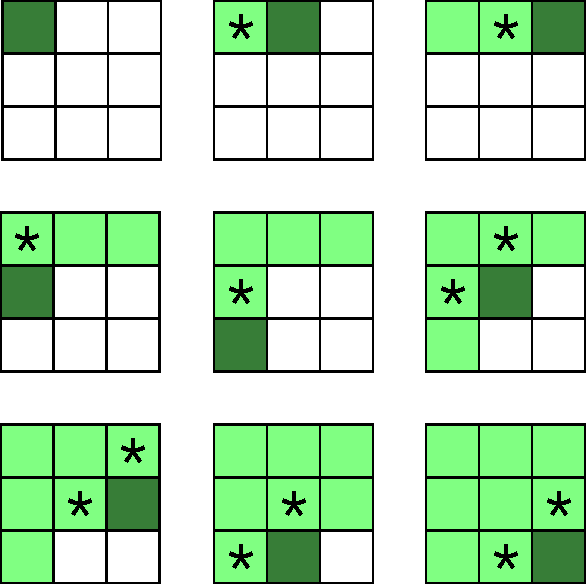
\includegraphics{imagenes/ej3_grilla_2.pdf}
		\caption{Visualización del cálculo de subsoluciones.}
	\end{figure}

	Por último, una vez que se tienen los valores finales de todos los
	casilleros calculados, se desea generar el camino buscado.

	Primero es necesario destacar que para cada posición de la
	grilla (además del costo) se guarda la dirección: \texttt{Y} corresponde a
	un salto horizontal, \texttt{X} vertical. De esta forma, al momento de
	construir el recorrido final, lo que se busca es tomar la dirección en la
	posición $(N, M)$ y dependiendo de la misma continuar el proceso
	en el casillero correspondiente ($(N, M - 1)$ si fuera \texttt{Y}, $(N - 1,
	M)$ caso contrario) guardando en cada paso la dirección tomada.

	Al finalizar se obtiene una secuencia con la dirección a tomar
	en cada paso para obtener el recorrido de costo óptimo.

	Todos los pasos descritos anteriormente se llevan a cabo mediante el siguiente algoritmo:

	\begin{algorithm}[H]
		\caption{Solución \emph{bottom-up} al problema}
		\Input{Una grilla $G$ de dimensiones $N \times M$ con la altura de cada
		casillero y un nivel de entrenamiento $H$.}
		\Output{Un par con el costo del camino óptimo de $(1, 1)$ a
		$(N, M)$ y su recorrido.}
		$DP$ $\gets$ grilla de dimensiones $N \times M$ donde cada elemento es
		un par del tipo entero y caracter \;
		$DP_{1,1}$ $\gets$ (0, 'I') \;
		\ForEach{$i$ entre $2$ y $N$}{
			$DP_{i,1}$ $\gets$ ($DP_{i-1,1} + $ costo del salto vertical, 'X') \;
		}
		\ForEach{$j$ entre $2$ y $M$}{
			$DP_{1,j}$ $\gets$ ($DP_{1,j-1} + $ costo del salto horizontal, 'Y') \;
		}
		\ForEach{$i$ entre $2$ y $N$ y $j$ entre $2$ y $M$}{
			$costoSaltoVertical$ $\gets$ $DP_{i-1,j} + $ costo del salto vertical \;
			$costoSaltoHorizontal$ $\gets$ $DP_{i,j-1} + $ costo del salto horizontal\;
			\eIf{$costoSaltoVertical < costoSaltoHorizontal$}{
				$DP_{i,j}$ $\gets$ ($costoSaltoVertical$, 'X') \;
			}
			{
				$DP_{i,j}$ $\gets$ ($costoSaltoHorizontal$, 'Y') \;
			}
		}
		$i$ $\gets$ $N$ \;
		$j$ $\gets$ $M$ \;
		$k$ $\gets$ $N + M - 2$ \;
		\While{$k > 0$}{
			$camino_k$ $\gets$ $DP_{i,j}$.segundo() \;
			\eIf{$DP_{i,j}$.segundo() es igual a 'Y'}{
				$j$ $\gets$ $j - 1$ \;
			}
			{
				$i$ $\gets$ $i - 1$ \;
			}
			$k$ $\gets$ $k - 1$ \;
		}
		\Return{($DP_{N,M}$, $camino$)}
	\end{algorithm}

    % Deducir una cota de complejidad temporal del algoritmo propuesto (en función de los parámetros que se consideren correctos) y justificar por qué el algoritmo la cumple. Utilizar el modelo uniforme.
    \subsection{Complejidad teórica}
	Inicializar la matriz de subsoluciones $DP$ de $N$ filas y $M$ columnas
	tiene un costo de $\ord(N \times M)$.

	Calcular el salto vertical u horizontal tiene un costo de $\ord(1)$.
	Calcular la primera fila tiene costo $\ord(M)$, ya que crece únicamente en
	función del tamaño de la fila la cantidad de operaciones constantes
	necesarias para calcular y almacenar en la matriz de subsoluciones ($DP$).
	Calcular la primera columna cuesta $\ord(N)$, ya que crece únicamente en
	función del tamaño de la columna el número de operaciones constantes
	necesarias.

    Para llenar el resto de la grilla $DP$, se la debe recorrer en orden creciente por columnas, a partir de la segunda fila y desde la segunda columna. En cada iteración se toma el mínimo entre dos valores: el costo del salto vertical más la subsolución correspondiente a la posición de arriba en la grilla, y el costo del salto horizontal más la subsolución correspondiente a la posición de la izquierda. Todas estas operaciones tienen un costo de $\ord(1)$, dando una complejidad total para terminar de llenar la grilla $DP$ de $\ord(N \times M)$.

    Para armar el camino, se va recorriendo la matriz desde la posición final, (fila $N - 1$ , columna $M - 1$) hasta la inicial (fila $0$ , columna $0$); en cada paso se consulta en la matriz $DP$ la dirección del movimiento correspondiente, se lo almacena, y se mueve a la siguiente posición (operaciones $\ord(1)$). Esto se repite un total de $N + M - 2$ iteraciones, ya que en cada paso corresponde a un movimiento a la izquierda o hacia arriba. Entonces, armar el camino cuesta $\ord(N + M - 2)$

    Por lo tanto, el costo total es $\ord( M + N + M \times N + (N + M - 2) ) = \ord(N \times M)$

    \subsection{Experimentación}
    El objetivo de la experimentación fue ver que la solución depende linealmente con respecto a $N$ y a $M$ y no depende de $H$.

    Para esto se realizaron cuatro experimentos:
    \begin{itemize}
        \item Variar $N$: Se varía entre 1 y 50000, con saltos de a 200 ($T_N$).
        \item Variar $M$: Se varía entre 1 y 50000, con saltos de a 200 ($T_M$).
        \item Variar $N$ y $M$: Se varía entre 1 y 1000, con saltos de a 10 ($T_{M \times N}$), $N$ y $M$ toman el mismo valor.
        \item Variar $H$: Se varía entre 1 y 50000, con saltos de a 200 ($T_H$), fijando el $M$ y el $N$ en $50000$.
    \end{itemize}

    \begin{figure}[H]
        \centering
        \caption{}
        \label{fig:exp3:var-nym-base}
        \begin{tikzpicture}
            \begin{axis}[
                    title={},
                    xlabel={Cantidad de filas ($N$) o de columnas ($M$)},
                    ylabel={Tiempo de ejecución (nanosegundos)},
                    scaled x ticks=false,
                    scaled y ticks=false,
                    enlargelimits=0.05,
                    width=0.5\textwidth,
                    height=0.5\textwidth,
                    legend pos=north west,
                    legend cell align=left,
                    xmin=100
                ]
                \addplot[color=green] table[x index=0,y index=1]{../exp/elRetornoDelJediFilas};
                \addplot[color=blue] table[x index=0,y index=1]{../exp/elRetornoDelJediColumnas};
                \addplot[color=red] table[x index=0, y expr={x*70}]{../exp/elRetornoDelJediFilas};
                \legend{$T_N$,$T_M$, $c \times N$}
            \end{axis}
        \end{tikzpicture}
    \end{figure}

	En el gráfico de la Figura \ref{fig:exp3:var-nym-base} se puede ver que al
	variar el valor de $N$ o de $M$, $T_N$ y $T_M$ son acotables por una recta
	con constante $c = 70$, lo cual prueba empíricamente la hipótesis de que la
	complejidad del algoritmo tiene una relación lineal con los valores tanto de
	$M$ como de $N$. Las rectas $T_N$ y $T_M$ difieren en la constante; esto se
	debe a las estructuras de datos utilizadas durante la resolución, ya que al
	aumentar el valor de $M$ se utiliza siempre un único vector grande, mientras
	que, al aumentar el $N$ se tienen $N$ vectores con un único elemento, lo
	cual hace que acceder al $i$-ésimo vector pueda volverse un poco más
	costoso, por ejemplo, porque los vectores podrían estar almacenados en
	lugares no contiguos de memoria.

    \begin{figure}[H]
        \centering
        \caption{}
        \label{fig:exp3:var-nym-divconst}
        \begin{tikzpicture}
            \begin{axis}[
                    title={},
                    xlabel={Cantidad de filas ($N$) o de columnas ($M$)},
                    ylabel={Tiempo de ejecución (nanosegundos)},
                    scaled x ticks=false,
                    scaled y ticks=false,
                    enlargelimits=0.05,
                    width=0.5\textwidth,
                    height=0.5\textwidth,
                    legend pos=north west,
                    legend cell align=left,
                    restrict x to domain=2000:50000,
                    ymax=200,
                    xmin=1
                ]
                \addplot[color=green] table[x index=0,y expr={\thisrowno{1}/x}]{../exp/elRetornoDelJediFilas};
                \addplot[color=blue] table[x index=0,y expr={\thisrowno{1}/x}]{../exp/elRetornoDelJediColumnas};
                \addplot[color=red] table[x index=0, y expr={70}]{../exp/elRetornoDelJediFilas};
                \legend{$T_N/N$,$T_M/M$,$c$}
            \end{axis}
        \end{tikzpicture}
    \end{figure}

	En el gráfico de la figura \ref{fig:exp3:var-nym-divconst}, se puede ver que
	si se lo divide por $N$ o $M$, el tiempo de ejecución queda acotable por la
	misma constante del gráfico anterior, lo cual confirma la linealidad de $T_N$ y $T_M$.
	\begin{figure}[H]
        \centering
        \caption{}
        \label{fig:exp3:var-nxn-base}
        \begin{tikzpicture}
            \begin{axis}[
                    title={},
                    xlabel={Tamaño de entrada ($N$)},
                    ylabel={Tiempo de ejecución (nanosegundos)},
                    scaled x ticks=false,
                    scaled y ticks=false,
                    enlargelimits=0.05,
                    width=0.5\textwidth,
                    height=0.5\textwidth,
                    legend pos=north west,
                    legend cell align=left,
                    xmin=1
                ]
                \addplot[color=black] table[x index=0,y index=1]{../exp/elRetornoDelJediFilasYColumnas};
                \addplot[color=red] table[x index=0, y expr={x*x*12}]{../exp/elRetornoDelJediFilasYColumnas};
                \legend{$T$, $cN^{2}$}
            \end{axis}
        \end{tikzpicture}
    \end{figure}

	En la Figura \ref{fig:exp3:var-nxn-base} se puede ver que al variar el $N$
	(y simultáneamente el $M$, ya que se considera $M = N$), $T_{M \times N}$ se
	puede acotar por una función cuadrática con constante $c = 12$.  \begin{figure}[H]
        \centering
        \caption{}
        \label{fig:exp3:var-nxn-divconst}
        \begin{tikzpicture}
            \begin{axis}[
                    title={},
                    xlabel={Tamaño de entrada ($N$)},
                    ylabel={Tiempo de ejecución (nanosegundos)},
                    scaled x ticks=false,
                    scaled y ticks=false,
                    enlargelimits=0.05,
                    width=0.5\textwidth,
                    height=0.5\textwidth,
                    legend pos=north west,
                    legend cell align=left,
                    restrict x to domain=5:1000,
                    xmin=1,
                    ymax=100
                ]
                \addplot[color=black] table[x index=0,y expr={\thisrowno{1}/(x*x)}]{../exp/elRetornoDelJediFilasYColumnas};
                \addplot[color=red] table[x index=0, y expr={12}]{../exp/elRetornoDelJediFilasYColumnas};
                \legend{$T_{M \times N}/N^{2}$, $c$}
            \end{axis}
        \end{tikzpicture}
    \end{figure}

    En el gráfico de la Figura \ref{fig:exp3:var-nxn-divconst} se puede ver que
	al dividir por $N^{2}$, queda acotable la misma constante que en el gráfico
	anterior, lo cual confirma que $T_{M \times N}$ tiene complejidad $O(M \times N)$.

    \begin{figure}[H]
        \centering
        \caption{}
        \label{fig:exp3:varh}
        \begin{tikzpicture}
            \begin{axis}[
                    title={},
                    xlabel={Nivel de entrenamiento de Luke ($H$)},
                    ylabel={Tiempo de ejecución (nanosegundos)},
                    scaled x ticks=false,
                    scaled y ticks=false,
                    enlargelimits=0.05,
                    width=0.5\textwidth,
                    height=0.5\textwidth,
                    legend pos=north west,
                    legend cell align=left,
                    restrict x to domain=0:48000,
                    xmin=1,
                    ymax=18000000
                ]
                \addplot[color=black] table[x index=0,y index=1]{../exp/elRetornoDelJediNivelDeEntrenamiento};
                \addplot[color=red] table[x index=0, y expr={13000000}]{../exp/elRetornoDelJediNivelDeEntrenamiento};
                \legend{$T_H$, $c$}
            \end{axis}
        \end{tikzpicture}
    \end{figure}

	En el gráfico de la Figura \ref{fig:exp3:varh}, por último, se puede ver que
	$T_H$ es acotable por por una constante ($c = 1.3 \times 10^7)$, lo cual corrobora que variar el $H$
	no afecta la complejidad del algoritmo.


\newpage
\appendix
\section{Apéndice: Código fuente de las funciones principales}\label{sec:codigo}

\subsection{Ejercicio 1 (Una nueva esperanza)}
\begin{lstlisting}
\end{lstlisting}

\subsection{Ejercicio 2 (El Imperio contraataca)}
\begin{lstlisting}
\end{lstlisting}

\subsection{Ejercicio 3 (El retorno del jedi)}
\begin{lstlisting}
\end{lstlisting}


\end{document}
